% !TeX program = xelatex
\documentclass[12pt,a4paper]{article}
\usepackage{fontspec}
\setmainfont{Times New Roman}[Path=C:/Windows/Fonts/,UprightFont=times.ttf,BoldFont=timesbd.ttf,ItalicFont=timesi.ttf,BoldItalicFont=timesbi.ttf]
\usepackage{amsmath,amssymb,amsfonts}
\usepackage[left=1.5cm,right=1.5cm,top=1.4cm,bottom=1.6cm,headheight=17pt]{geometry}
\usepackage{enumitem,array,graphicx,tikz,fancyhdr,needspace}
\usetikzlibrary{arrows.meta,calc,patterns}
% Sửa số đề và số trang đề thực tế sau khi biên dịch/tách PDF.
\newcommand{\soDe}{8}
\newcommand{\soTrangDe}{4}
\newcommand{\maDe}{\ifnum\soDe<1000 0\fi\ifnum\soDe<100 0\fi\ifnum\soDe<10 0\fi\soDe}
\pagestyle{fancy}
\fancyhf{}
\lhead{\small\textbf{ÔN TẬP GIỮA KÌ I}}
\rhead{\small\textit{Biên soạn: Dương Gia Bảo}}
\rfoot{\small Trang \thepage/\soTrangDe\ - Mã đề: \maDe}
\renewcommand{\headrulewidth}{0.4pt}
\fancypagestyle{answers}{\rfoot{\small Trang \thepage\ - Mã đề: \maDe}}
\fancypagestyle{firstpage}{\fancyhead{}\renewcommand{\headrulewidth}{0pt}}
\setlength{\parindent}{0pt}
\setlength{\parskip}{2.5pt}
\setlength{\emergencystretch}{1em}
\setlist[enumerate,1]{label=\textbf{Câu \arabic*:},leftmargin=*,itemsep=5pt,topsep=2pt}
\setlist[enumerate,2]{label=\alph*),leftmargin=*,itemsep=2pt,topsep=2pt}
\newcommand{\bonpa}[4]{\par\nobreak\smallskip\nobreak\noindent
\begin{tabular}{@{}p{0.47\linewidth}p{0.47\linewidth}@{}}
\textbf{A.} #1 & \textbf{B.} #2\\[8pt]
\textbf{C.} #3 & \textbf{D.} #4\end{tabular}}
\newcommand{\loigiai}[1]{\par\medskip\Needspace{4\baselineskip}\noindent\textbf{#1}\par\nobreak}
\newcommand{\otraloi}{\par\nobreak\smallskip\noindent\textit{Trả lời:}\quad\fbox{\rule{0pt}{11pt}\makebox[0.3cm]{}}\,\fbox{\rule{0pt}{11pt}\makebox[0.3cm]{}}\,\fbox{\rule{0pt}{11pt}\makebox[0.3cm]{}}\,\fbox{\rule{0pt}{11pt}\makebox[0.3cm]{}}}
\begin{document}
\thispagestyle{firstpage}
\noindent
\begin{minipage}[t]{0.35\textwidth}
    \centering
    {\fontsize{13}{15}\selectfont\textbf{ÔN TẬP GIỮA KÌ I}}\\[4pt]
    \textit{Biên soạn: Dương Gia Bảo}\\[5pt]
    \setlength{\fboxrule}{0.8pt}%
    \setlength{\fboxsep}{4pt}%
    \fbox{\begin{minipage}{0.83\linewidth}
        \centering
        {\fontsize{13}{15}\selectfont\textbf{ĐỀ ÔN TẬP}\\[2pt]\textbf{CHƯƠNG I VÀ II}}\\[4pt]
        \textit{(Đề thi gồm có \ifnum\soTrangDe<10 0\fi\soTrangDe\ trang)}
    \end{minipage}}
\end{minipage}\hfill
\begin{minipage}[t]{0.63\textwidth}
    \centering
    {\fontsize{13}{15}\selectfont\textbf{ÔN TẬP KIỂM TRA GIỮA KÌ I}\\[2pt]
    \textbf{NĂM HỌC 2026 - 2027}}\\[5pt]
    {\fontsize{14}{16}\selectfont\textbf{Môn: TOÁN - Lớp 12 (ĐỀ SỐ \soDe)}}\\[4pt]
    {\fontsize{11.5}{13}\selectfont\textit{Thời gian làm bài: 90 phút, không kể thời gian giao đề}}\\[5pt]
    \setlength{\fboxrule}{0.8pt}%
    \setlength{\fboxsep}{5pt}%
    \fbox{\makebox[3cm]{\fontsize{14}{16}\selectfont\textbf{Mã đề: \maDe}}}
\end{minipage}
\par\vspace{2pt}
\hrule height 0.6pt
\vspace{3pt}
\noindent\textit{Họ và tên học sinh:}\dotfill\hspace{1cm}\textit{Lớp:}\makebox[3.5cm]{\dotfill}
\par\vspace{2pt}
\hrule height 0.6pt
\vspace{3pt}

\section*{\large PHẦN I. Câu trắc nghiệm nhiều phương án lựa chọn}
\textit{Thí sinh trả lời từ câu 1 đến câu 12. Mỗi câu chỉ chọn một phương án.}
\begin{enumerate}
\item Cho hàm số $y=-x^3+3x+1$. Hàm số đã cho đồng biến trên khoảng nào dưới đây?
\bonpa{$(-1;1)$.}{$(-\infty;-1)$.}{$(1;+\infty)$.}{$(0;2)$.}

\item Cho hàm số $y=2x^3-3x^2-12x+5$. Điểm cực tiểu của hàm số đã cho là
\bonpa{$x=-1$.}{$x=5$.}{$x=2$.}{$x=-15$.}

\item Giá trị nhỏ nhất của hàm số $f(x)=x^3-3x+5$ trên đoạn $[0;2]$ bằng
\bonpa{$5$.}{$3$.}{$7$.}{$1$.}

\item Đường tiệm cận đứng và đường tiệm cận ngang của đồ thị hàm số $y=\dfrac{2x-3}{x-1}$ lần lượt có phương trình là
\bonpa{$x=2$ và $y=1$.}{$x=-1$ và $y=2$.}{$x=1$ và $y=-3$.}{$x=1$ và $y=2$.}

\item Đường tiệm cận xiên của đồ thị hàm số $y=\dfrac{x^2+2x-1}{x+1}$ có phương trình là
\bonpa{$y=x-1$.}{$y=x+2$.}{$y=x+1$.}{$y=2x+1$.}

\item Đường cong trong hình vẽ bên là đồ thị của hàm số nào dưới đây?
\par\nobreak\smallskip
\begin{minipage}[c]{0.62\linewidth}
\bonpa{$y=\dfrac{x^2-x+1}{x-1}$.}{$y=\dfrac{x^2+x+1}{x+1}$.}{$y=\dfrac{x^2-2x+2}{x-1}$.}{$y=\dfrac{x^2+1}{x-1}$.}
\end{minipage}\hfill
\begin{minipage}[c]{0.36\linewidth}\centering
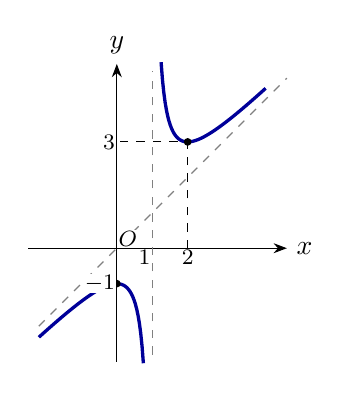
\begin{tikzpicture}[x=0.45cm,y=0.45cm,>=Stealth]
\draw[->] (-2.5,0)--(4.8,0) node[right] {$x$};
\draw[->] (0,-3.2)--(0,5.2) node[above] {$y$};
\draw[dashed,gray] (1,-3.0)--(1,5.0);
\draw[dashed,gray] (-2.2,-2.2)--(4.8,4.8);
\draw[very thick,blue!60!black,domain=-2.2:0.75,samples=80] plot (\x,{(\x*\x-\x+1)/(\x-1)});
\draw[very thick,blue!60!black,domain=1.25:4.2,samples=80] plot (\x,{(\x*\x-\x+1)/(\x-1)});
\draw[dashed] (2,0)--(2,3)--(0,3);
\fill (0,-1) circle (1.4pt);
\fill (2,3) circle (1.4pt);
\node[above right,fill=white,inner sep=0.5pt] at (0,0) {\footnotesize $O$};
\node[below left,fill=white,inner sep=0.5pt] at (1,0) {\footnotesize $1$};
\node[below,fill=white,inner sep=0.5pt] at (2,0) {\footnotesize $2$};
\node[left,fill=white,inner sep=0.5pt] at (0,-1) {\footnotesize $-1$};
\node[left,fill=white,inner sep=0.5pt] at (0,3) {\footnotesize $3$};
\end{tikzpicture}
\end{minipage}
\end{enumerate}

\newpage
\begin{enumerate}[start=7]
\item Số lượng sản phẩm bán ra của một công ty phụ thuộc vào giá bán $p$ (nghìn đồng) theo công thức $D(p)=1200-20p$ với $10\le p\le 50$. Doanh thu từ việc bán sản phẩm là $R(p)=p\cdot D(p)=1200p-20p^2$. Để doanh thu đạt giá trị lớn nhất thì giá bán $p$ bằng bao nhiêu nghìn đồng?
\bonpa{$25$.}{$30$.}{$35$.}{$40$.}

\item Cho hình hộp $ABCD.A'B'C'D'$. Tổng ba vectơ $\vec{BA}+\vec{BC}+\vec{BB'}$ bằng vectơ nào dưới đây?
\bonpa{$\vec{BD}$.}{$\vec{AC'}$.}{$\vec{B'D}$.}{$\vec{BD'}$.}

\item Trong không gian $Oxyz$, cho hai điểm $A(1;2;-3)$ và $B(3;-4;1)$. Tọa độ trung điểm $M$ của đoạn thẳng $AB$ là
\bonpa{$(2;-1;-1)$.}{$(4;-2;-2)$.}{$(1;-3;2)$.}{$(-2;1;1)$.}

\item Trong không gian $Oxyz$, cho hai vectơ $\vec{a}=(2;-1;3)$ và $\vec{b}=(-1;2;1)$. Tọa độ của vectơ $\vec{u}=3\vec{a}-2\vec{b}$ là
\bonpa{$(4;-7;7)$.}{$(8;1;11)$.}{$(8;-7;7)$.}{$(4;-1;7)$.}

\item Trong không gian $Oxyz$, cho hai vectơ $\vec{u}=(1;-2;2)$ và $\vec{v}=(3;1;-2)$. Tích vô hướng $\vec{u}\cdot\vec{v}$ bằng
\bonpa{$-1$.}{$-3$.}{$3$.}{$-5$.}

\item Trong không gian $Oxyz$, cho hai điểm $A(2;1;-1)$ và $B(0;3;-2)$. Độ dài đoạn thẳng $AB$ bằng
\bonpa{$\sqrt{5}$.}{$9$.}{$\sqrt{13}$.}{$3$.}
\end{enumerate}

\vspace{3pt}
\section*{\large PHẦN II. Câu trắc nghiệm đúng hoặc sai}
\textit{Thí sinh trả lời từ câu 1 đến câu 4. Trong mỗi ý a), b), c), d) ở mỗi câu, thí sinh chọn đúng hoặc sai.}
\begin{enumerate}
\item Cho hàm số $y=f(x)=\dfrac{x^2-4x+5}{x-2}$.
\begin{enumerate}
\item Tập xác định của hàm số là $D=\mathbb{R}\setminus\{2\}$.
\item Đạo hàm của hàm số là $f'(x)=\dfrac{x^2-4x+3}{(x-2)^2}$.
\item Đồ thị hàm số có đường tiệm cận xiên là đường thẳng $y=x+2$.
\item Đồ thị hàm số có hai điểm cực trị $A$ và $B$. Độ dài đoạn thẳng $AB$ bằng $2\sqrt{5}$.
\end{enumerate}
\end{enumerate}

\newpage
\begin{enumerate}[start=2]
\item Một công ty công nghệ sản xuất một thiết bị thông minh với số lượng $x$ nghìn thiết bị trong một tháng ($0 < x \le 50$). Tổng chi phí sản xuất (tính bằng triệu đồng) được cho bởi hàm số $C(x)=x^3-40x^2+600x+1000$. Doanh thu từ việc bán thiết bị (tính bằng triệu đồng) được cho bởi hàm số $R(x)=1500x-10x^2$. Lợi nhuận của công ty là $P(x)=R(x)-C(x)$.
\begin{enumerate}
\item Chi phí cố định ban đầu của công ty (khi chưa sản xuất thiết bị nào) là $1000$ triệu đồng.
\item Doanh thu của công ty khi bán được $20$ nghìn thiết bị là $26000$ triệu đồng.
\item Hàm lợi nhuận của công ty theo số lượng $x$ là $P(x)=-x^3+30x^2+900x-1000$.
\item Doanh nghiệp đạt lợi nhuận lớn nhất trong tháng khi sản xuất $25$ nghìn thiết bị.
\end{enumerate}

\item Trong không gian $Oxyz$, cho ba điểm $A(1;0;2)$, $B(2;2;1)$ và $C(-1;2;4)$.
\begin{enumerate}
\item Tọa độ của vectơ $\vec{AB}$ là $\vec{AB}=(1;2;-1)$.
\item Trọng tâm $G$ của tam giác $ABC$ có tọa độ là $G\left(\dfrac{2}{3};\dfrac{4}{3};\dfrac{7}{3}\right)$.
\item Tích vô hướng $\vec{AB}\cdot\vec{AC}=0$, suy ra tam giác $ABC$ vuông tại $A$.
\item Tọa độ điểm $D$ để tứ giác $ABCD$ là hình bình hành là $D(-2;0;3)$.
\end{enumerate}

\item Một chùm đèn trang trí nghệ thuật có trọng lượng $P=150\text{ N}$ được treo vào trần nhà bằng ba sợi dây cáp mảnh, không dãn, có độ dài bằng nhau. Ba đầu dây trên trần nhà được cố định tại ba điểm $A, B, C$ tạo thành một tam giác đều nằm trên mặt phẳng nằm ngang, và cùng được buộc vào móc treo chùm đèn tại điểm $O$. Chọn hệ trục toạ độ $Oxyz$ có gốc tại $O$, tia $Oz$ hướng thẳng đứng lên trần nhà (ngược hướng với trọng lực). Khi đó trọng lực tác dụng lên chùm đèn là $\vec{P}=(0;0;-150)$ (đơn vị: N). Lực căng của ba sợi dây tác dụng lên móc treo $O$ lần lượt là $\vec{F}_1, \vec{F}_2, \vec{F}_3$. Biết rằng ba lực $\vec{F}_1, \vec{F}_2, \vec{F}_3$ có độ lớn bằng nhau $|\vec{F}_1|=|\vec{F}_2|=|\vec{F}_3|=F$, cùng tạo với phương thẳng đứng (trục $Oz$) một góc $60^\circ$, và hình chiếu của ba lực lên mặt phẳng nằm ngang $Oxy$ đôi một hợp với nhau một góc $120^\circ$.
\begin{enumerate}
\item Vì chùm đèn ở trạng thái cân bằng nên ta có hệ thức $\vec{F}_1+\vec{F}_2+\vec{F}_3+\vec{P}=\vec{0}$.
\item Hợp lực của ba lực căng dây $\vec{F}=\vec{F}_1+\vec{F}_2+\vec{F}_3$ có phương thẳng đứng hướng lên, cùng hướng với vectơ đơn vị $\vec{k}$ của trục $Oz$.
\item Độ lớn của mỗi lực căng dây là $F=100\text{ N}$.
\item Góc tạo bởi mỗi sợi dây cáp và mặt phẳng nằm ngang của trần nhà bằng $60^\circ$.
\end{enumerate}
\end{enumerate}

\vspace{3pt}
\section*{\large PHẦN III. Câu trắc nghiệm trả lời ngắn}
\textit{Thí sinh trả lời từ câu 1 đến câu 6. Mỗi câu trả lời đúng thí sinh được 0,5 điểm.}
\begin{enumerate}
\item Tìm số giá trị nguyên của tham số $m\in[-10;10]$ để hàm số $y=\dfrac{1}{3}x^3-(m-1)x^2+(m+5)x-2026$ đồng biến trên khoảng $(-\infty;+\infty)$.
\otraloi

\item Trong không gian $Oxyz$, cho hình hộp $ABCD.A'B'C'D'$ có tọa độ các đỉnh $A(1;0;1)$, $B(2;1;2)$, $D(1;-1;3)$ và $A'(4;2;1)$. Tìm tọa độ đỉnh $C'(x;y;z)$, sau đó tính tổng $S=x+y+z$.
\otraloi
\end{enumerate}

\newpage
\begin{enumerate}[start=3]
\item Cho hàm số $y=\dfrac{x^2+mx+1}{x-1}$ ($m$ là tham số thực). Có bao nhiêu giá trị nguyên của tham số $m\in[-8;8]$ để đồ thị hàm số có hai điểm cực trị nằm về hai phía của trục tung?
\otraloi

\item Trong không gian $Oxyz$ (với đơn vị đo trên các trục là mét), có hai thiết bị bay không người lái (drone) $A$ và $B$ đang bay thử nghiệm. Tại thời điểm $t$ giây ($t\ge 0$), vị trí của drone $A$ là $A(t;6;7)$ và vị trí của drone $B$ là $B(3t;2t;t+1)$. Khoảng cách ngắn nhất giữa hai drone trong quá trình bay bằng bao nhiêu mét?
\otraloi

\item Người ta muốn làm một chiếc bể chứa nước bằng tôn không nắp dạng hình hộp chữ nhật có thể tích bằng $32\text{ m}^3$. Đáy bể là hình vuông có cạnh bằng $x\text{ m}$, chiều cao của bể là $h\text{ m}$ (hình vẽ minh họa). Để tiết kiệm vật liệu nhất, diện tích toàn phần (không nắp) của bể phải đạt giá trị nhỏ nhất. Hỏi diện tích toàn phần nhỏ nhất của bể bằng bao nhiêu mét vuông?
\begin{center}
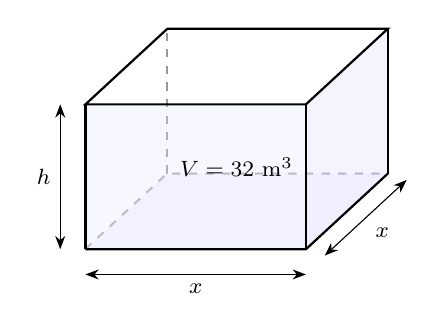
\begin{tikzpicture}[x=0.8cm,y=0.8cm,>=Stealth]
\coordinate (A) at (0,0);
\coordinate (B) at (3.5,0);
\coordinate (C) at (4.8,1.2);
\coordinate (D) at (1.3,1.2);
\coordinate (A1) at (0,2.3);
\coordinate (B1) at (3.5,2.3);
\coordinate (C1) at (4.8,3.5);
\coordinate (D1) at (1.3,3.5);

\draw[dashed,thick,gray!80] (A)--(D)--(C);
\draw[dashed,thick,gray!80] (D)--(D1);

\fill[blue!5,opacity=0.5] (A)--(B)--(C)--(D)--cycle;
\fill[blue!10,opacity=0.3] (A)--(B)--(B1)--(A1)--cycle;
\fill[blue!15,opacity=0.3] (B)--(C)--(C1)--(B1)--cycle;

\draw[thick] (A)--(B)--(C);
\draw[thick] (A1)--(B1)--(C1)--(D1)--cycle;
\draw[thick] (A)--(A1) (B)--(B1) (C)--(C1);

\draw[<->] (0,-0.4)--(3.5,-0.4) node[midway,below] {\footnotesize $x$};
\draw[<->] (3.8,-0.1)--(5.1,1.1) node[midway,below right] {\footnotesize $x$};
\draw[<->] (-0.4,0)--(-0.4,2.3) node[midway,left] {\footnotesize $h$};

\node at (2.4,1.3) {\footnotesize $V = 32\text{ m}^3$};
\end{tikzpicture}
\par\smallskip{\footnotesize\textit{Hình minh họa bể nước không nắp.}}
\end{center}
\otraloi

\item Một nhà máy phát điện $P$ nằm trên bờ biển thẳng cần truyền tải điện đến một trạm biến áp trên một hòn đảo $A$. Khoảng cách từ đảo $A$ đến bờ biển là $AH=4\text{ km}$ ($H$ là hình chiếu vuông góc của $A$ lên đường bờ biển thẳng). Khoảng cách từ nhà máy $P$ đến điểm $H$ dọc theo bờ biển là $PH=10\text{ km}$. Người ta dự định kéo đường dây điện gồm hai đoạn: đoạn dây trên bờ chạy dọc theo bờ biển từ $P$ đến điểm $C$ (với $C$ nằm giữa $P$ và $H$), và đoạn cáp ngầm đi dưới biển nối từ $C$ đến đảo $A$ (hình vẽ minh họa). Biết chi phí lắp đặt mỗi kilômét đường dây trên bờ là $30$ triệu đồng, chi phí lắp đặt mỗi kilômét cáp ngầm dưới biển là $50$ triệu đồng. Tổng chi phí lắp đặt nhỏ nhất của toàn bộ đường dây điện bằng bao nhiêu triệu đồng?
\begin{center}
\begin{tikzpicture}[x=0.70cm,y=0.70cm,>=Stealth]
\draw[thick,blue!50!gray] (-0.5,0)--(11.0,0) node[above,black] {\footnotesize Đường bờ biển};
\fill[cyan!10] (-0.5,-2.7) rectangle (11.0,0);
\node at (4.5,-1.8) {\textit{\footnotesize Biển}};
\node at (4.5,0.7) {\textit{\footnotesize Đất liền}};

\coordinate (P) at (0.5,0);
\coordinate (H) at (10.0,0);
\coordinate (C) at (7.0,0);
\coordinate (A) at (10.0,-2.5);

\fill (P) circle (2pt) node[above] {$P$};
\fill (H) circle (2pt) node[above] {$H$};
\fill (C) circle (2pt) node[above] {$C$};
\fill (A) circle (2pt) node[below] {$A$};

\draw[dashed] (A)--(H);
\draw (10.0,-0.3)--(9.7,-0.3)--(9.7,0);
\draw[line width=1.5pt,orange!80!black] (P)--(C) node[midway,above] {\footnotesize Dây trên bờ};
\draw[line width=1.4pt,red!80!black] (C)--(A) node[midway,below left] {\footnotesize Cáp ngầm};

\draw[<->] (0.5,0.4)--(10.0,0.4) node[midway,above] {\footnotesize $10\text{ km}$};
\draw[<->] (10.5,0)--(10.5,-2.5) node[midway,right] {\footnotesize $4\text{ km}$};
\draw[<->] (7.0,-0.3)--(10.0,-0.3) node[midway,below] {\footnotesize $x$};
\end{tikzpicture}
\par\smallskip{\footnotesize\textit{Sơ đồ phương án kéo đường dây điện.}}
\end{center}
\otraloi
\end{enumerate}
\begin{center}\textbf{---------------- HẾT ----------------}\end{center}

\newpage\pagestyle{answers}
\begin{center}\Large\textbf{BẢNG ĐÁP ÁN TỔNG HỢP}\end{center}
\textbf{Phần I. Trắc nghiệm nhiều phương án lựa chọn}
\begin{center}
\renewcommand{\arraystretch}{1.5}
\begin{tabular}{|c|*{12}{c|}}\hline
Câu & 1&2&3&4&5&6&7&8&9&10&11&12\\\hline
Đáp án & A & C & B & D & C & A & B & D & A & C & B & D \\\hline
\end{tabular}
\end{center}

\textbf{Phần II. Đúng hoặc sai}
\begin{center}
\renewcommand{\arraystretch}{1.4}
\begin{tabular}{|c|c|c|c|c|}\hline
Câu & a) & b) & c) & d)\\\hline
1 & Đ & Đ & S & Đ\\\hline
2 & Đ & Đ & Đ & S\\\hline
3 & Đ & Đ & Đ & S\\\hline
4 & Đ & Đ & Đ & S\\\hline
\end{tabular}
\end{center}

\textbf{Phần III. Trả lời ngắn}
\begin{center}
\renewcommand{\arraystretch}{1.5}
\begin{tabular}{|c|c|c|c|c|c|c|}\hline
Câu & 1 & 2 & 3 & 4 & 5 & 6\\\hline
Đáp án & 6 & 11 & 9 & 6 & 48 & 460 \\\hline
\end{tabular}
\end{center}

\vspace{0.5cm}
\begin{center}
\large\textbf{HƯỚNG DẪN GIẢI CHI TIẾT}
\end{center}

\section*{PHẦN I}

\loigiai{Câu 1. Chọn A.}
Hàm số đã cho là $y=-x^3+3x+1$.
Tập xác định: $D=\mathbb{R}$.
Đạo hàm: $y'=-3x^2+3=-3(x^2-1)$.
Ta có $y'>0 \iff x^2-1 < 0 \iff -1 < x < 1$.
Do đó, hàm số đồng biến trên khoảng $(-1;1)$.

\loigiai{Câu 2. Chọn C.}
Hàm số đã cho là $y=2x^3-3x^2-12x+5$.
Tập xác định: $D=\mathbb{R}$.
Đạo hàm: $y'=6x^2-6x-12=6(x^2-x-2)$.
$y'=0 \iff x=-1$ hoặc $x=2$.
Đạo hàm cấp hai: $y''=12x-6$.
Tại $x=2$: $y''(2)=12(2)-6=18>0 \implies x=2$ là điểm cực tiểu của hàm số.

\loigiai{Câu 3. Chọn B.}
Hàm số $f(x)=x^3-3x+5$ liên tục trên $[0;2]$.
Đạo hàm: $f'(x)=3x^2-3$.
$f'(x)=0 \iff x^2=1 \iff x=1$ (do $x\in[0;2]$).
Tính các giá trị tại các điểm biên và điểm dừng:
$f(0)=5$; $f(1)=1-3+5=3$; $f(2)=8-6+5=7$.
Vậy giá trị nhỏ nhất của hàm số trên đoạn $[0;2]$ bằng $3$ (đạt tại $x=1$).

\loigiai{Câu 4. Chọn D.}
Hàm số $y=\dfrac{2x-3}{x-1}$.
Vì $\lim_{x\to 1^+} \dfrac{2x-3}{x-1} = -\infty$ nên đồ thị hàm số có tiệm cận đứng là $x=1$.
Vì $\lim_{x\to +\infty} \dfrac{2x-3}{x-1} = 2$ nên đồ thị hàm số có tiệm cận ngang là $y=2$.

\loigiai{Câu 5. Chọn C.}
Ta thực hiện phép chia đa thức:
$x^2+2x-1 = x(x+1) + (x+1) - 2 = (x+1)^2 - 2$.
Suy ra $y = x+1 - \dfrac{2}{x+1}$.
Vì $\lim_{x\to \pm\infty} [y - (x+1)] = \lim_{x\to \pm\infty} \left(-\dfrac{2}{x+1}\right) = 0$ nên đường thẳng $y=x+1$ là đường tiệm cận xiên của đồ thị hàm số.

\loigiai{Câu 6. Chọn A.}
Đồ thị hàm số có đường tiệm cận đứng là $x=1$ và đường tiệm cận xiên là $y=x$.
Đồ thị cắt trục tung tại điểm $(0;-1)$, đạt cực đại tại $(0;-1)$ và cực tiểu tại $(2;3)$.
Xét hàm số ở phương án A: $y=\dfrac{x^2-x+1}{x-1} = x + \dfrac{1}{x-1}$.
- Tiệm cận đứng: $x=1$; tiệm cận xiên: $y=x$.
- Điểm cắt trục tung: $x=0 \implies y=-1$.
- $y'=1-\dfrac{1}{(x-1)^2} = \dfrac{x(x-2)}{(x-1)^2} = 0 \iff x=0$ hoặc $x=2$.
- Cực đại tại $(0;-1)$ và cực tiểu tại $(2;3)$.
Vậy đồ thị đã cho là đồ thị của hàm số $y=\dfrac{x^2-x+1}{x-1}$.

\loigiai{Câu 7. Chọn B.}
Hàm doanh thu $R(p)=1200p-20p^2$ với $10\le p\le 50$.
Đạo hàm: $R'(p)=1200-40p$.
$R'(p)=0 \iff p=30\in[10;50]$.
Vì hệ số $a=-20<0$ nên hàm số $R(p)$ đạt giá trị lớn nhất tại đỉnh parabol $p=30$.
Vậy để doanh thu lớn nhất thì giá bán là $30$ nghìn đồng.

\loigiai{Câu 8. Chọn D.}
Áp dụng quy tắc hình bình hành cho đáy $ABCD$: $\vec{BA}+\vec{BC}=\vec{BD}$.
Tiếp tục áp dụng quy tắc hình bình hành cho mặt phẳng $(BDD'B')$:
$\vec{BD}+\vec{BB'}=\vec{BD'}$.
Do đó, theo quy tắc hình hộp: $\vec{BA}+\vec{BC}+\vec{BB'}=\vec{BD'}$.

\loigiai{Câu 9. Chọn A.}
Tọa độ trung điểm $M$ của đoạn thẳng $AB$ là:
$x_M=\dfrac{x_A+x_B}{2}=\dfrac{1+3}{2}=2$,
$y_M=\dfrac{y_A+y_B}{2}=\dfrac{2+(-4)}{2}=-1$,
$z_M=\dfrac{z_A+z_B}{2}=\dfrac{-3+1}{2}=-1$.
Vậy $M(2;-1;-1)$.

\loigiai{Câu 10. Chọn C.}
Ta có $3\vec{a}=3(2;-1;3)=(6;-3;9)$ và $2\vec{b}=2(-1;2;1)=(-2;4;2)$.
Suy ra $\vec{u}=3\vec{a}-2\vec{b}=(6-(-2); -3-4; 9-2)=(8;-7;7)$.

\loigiai{Câu 11. Chọn B.}
Tích vô hướng của hai vectơ $\vec{u}$ và $\vec{v}$ là:
$\vec{u}\cdot\vec{v}=1\cdot 3 + (-2)\cdot 1 + 2\cdot(-2) = 3 - 2 - 4 = -3$.

\loigiai{Câu 12. Chọn D.}
Ta có $\vec{AB}=(0-2; 3-1; -2-(-1))=(-2;2;-1)$.\\
Độ dài đoạn thẳng $AB$ là:
$AB = \sqrt{(-2)^2+2^2+(-1)^2} = \sqrt{4+4+1} = \sqrt{9}=3$.

\newpage
\section*{PHẦN II}

\loigiai{Câu 1.}
Cho hàm số $y=f(x)=\dfrac{x^2-4x+5}{x-2}$.
\begin{enumerate}
\item \textbf{Đúng.} Hàm số xác định khi và chỉ khi mẫu số khác 0, tức $x-2\ne 0 \iff x\ne 2$. Do đó $D=\mathbb{R}\setminus\{2\}$.
\item \textbf{Đúng.} Ta có $f'(x)=\dfrac{(2x-4)(x-2)-(x^2-4x+5)}{(x-2)^2} = \dfrac{2(x-2)^2-(x^2-4x+5)}{(x-2)^2} = \dfrac{2x^2-8x+8-x^2+4x-5}{(x-2)^2} = \dfrac{x^2-4x+3}{(x-2)^2}$.
\item \textbf{Sai.} Phép chia đa thức cho ta $f(x)=x-2+\dfrac{1}{x-2}$. Vì $\lim_{x\to \pm\infty}[f(x)-(x-2)]=0$ nên đường tiệm cận xiên là $y=x-2$, chứ không phải $y=x+2$.
\item \textbf{Đúng.} Phương trình $f'(x)=0 \iff x^2-4x+3=0 \iff x=1$ hoặc $x=3$.
Với $x=1 \implies y=-2$, ta được điểm cực đại $A(1;-2)$.
Với $x=3 \implies y=2$, ta được điểm cực tiểu $B(3;2)$.
Độ dài $AB=\sqrt{(3-1)^2+(2-(-2))^2}=\sqrt{4+16}=\sqrt{20}=2\sqrt{5}$.
\end{enumerate}

\loigiai{Câu 2.}
Cho $C(x)=x^3-40x^2+600x+1000$ và $R(x)=1500x-10x^2$ với $0<x\le 50$.
\begin{enumerate}
\item \textbf{Đúng.} Khi $x=0$, chi phí cố định là $C(0)=1000$ triệu đồng.
\item \textbf{Đúng.} Khi bán được 20 nghìn thiết bị ($x=20$), doanh thu là:
$R(20)=1500(20)-10(20^2)=30000-4000=26000$ triệu đồng.
\item \textbf{Đúng.} Hàm lợi nhuận:
$P(x)=R(x)-C(x)=(1500x-10x^2)-(x^3-40x^2+600x+1000)=-x^3+30x^2+900x-1000$.
\item \textbf{Sai.} Ta tính $P'(x)=-3x^2+60x+900=-3(x^2-20x-300)=-3(x-30)(x+10)$.
Trên khoảng $(0;50]$, $P'(x)=0 \iff x=30$.
Bảng biến thiên cho thấy hàm số $P(x)$ đồng biến trên $(0;30)$ và nghịch biến trên $(30;50)$.
Do đó lợi nhuận lớn nhất đạt được khi công ty sản xuất $30$ nghìn thiết bị, không phải $25$ nghìn thiết bị.
\end{enumerate}

\loigiai{Câu 3.}
Cho $A(1;0;2)$, $B(2;2;1)$ và $C(-1;2;4)$.
\begin{enumerate}
\item \textbf{Đúng.} Ta có $\vec{AB}=(2-1; 2-0; 1-2)=(1;2;-1)$.
\item \textbf{Đúng.} Tọa độ trọng tâm $G$ của tam giác $ABC$ là:
$x_G=\dfrac{1+2-1}{3}=\dfrac{2}{3}$, $y_G=\dfrac{0+2+2}{3}=\dfrac{4}{3}$, $z_G=\dfrac{2+1+4}{3}=\dfrac{7}{3}$.
Vậy $G\left(\dfrac{2}{3};\dfrac{4}{3};\dfrac{7}{3}\right)$.
\item \textbf{Đúng.} Ta có $\vec{AC}=(-1-1; 2-0; 4-2)=(-2;2;2)$.
Tích vô hướng: $\vec{AB}\cdot\vec{AC}=1\cdot(-2)+2\cdot 2+(-1)\cdot 2=-2+4-2=0$.
Do đó $\vec{AB}\perp\vec{AC}$, suy ra tam giác $ABC$ vuông tại $A$.
\item \textbf{Sai.} Tứ giác $ABCD$ là hình bình hành khi và chỉ khi $\vec{AD}=\vec{BC}$.
Ta có $\vec{BC}=(-1-2; 2-2; 4-1)=(-3;0;3)$.
Gọi $D(x_D;y_D;z_D) \implies \vec{AD}=(x_D-1; y_D; z_D-2)$.
$\vec{AD}=\vec{BC} \iff \begin{cases} x_D-1=-3 \\ y_D=0 \\ z_D-2=3 \end{cases} \iff \begin{cases} x_D=-2 \\ y_D=0 \\ z_D=5 \end{cases}$.
Vậy tọa độ đỉnh $D$ phải là $D(-2;0;5)$, không phải $D(-2;0;3)$.
\end{enumerate}

\loigiai{Câu 4.}
Chùm đèn có trọng lượng $P=150\text{ N}$, treo bởi 3 sợi dây cân bằng.
\begin{enumerate}
\item \textbf{Đúng.} Theo định luật I Newton, khi vật ở trạng thái cân bằng thì tổng các lực tác dụng lên vật bằng vectơ không: $\vec{F}_1+\vec{F}_2+\vec{F}_3+\vec{P}=\vec{0}$.
\item \textbf{Đúng.} Do tính chất đối xứng của ba điểm treo $A, B, C$ tạo thành tam giác đều và ba lực cùng tạo góc $60^\circ$ với phương thẳng đứng, các thành phần nằm ngang của ba lực triệt tiêu lẫn nhau từng đôi một: tổng hình chiếu lên mặt phẳng $Oxy$ bằng $\vec{0}$. Do đó hợp lực $\vec{F}=\vec{F}_1+\vec{F}_2+\vec{F}_3$ có phương thẳng đứng, hướng lên trên, cùng hướng với vectơ đơn vị $\vec{k}$ của trục $Oz$.
\item \textbf{Đúng.} Chiếu phương trình cân bằng lên trục $Oz$ theo chiều hướng lên:
$|\vec{F}_1|\cos 60^\circ + |\vec{F}_2|\cos 60^\circ + |\vec{F}_3|\cos 60^\circ - P = 0$.
Vì ba lực căng có cùng độ lớn $F$ nên:
$3F\cos 60^\circ = 150 \iff 3F\cdot 0{,}5 = 150 \iff 1{,}5 F = 150 \iff F=100\text{ N}$.
\item \textbf{Sai.} Vì mỗi sợi dây cáp tạo với phương thẳng đứng (trục $Oz$) một góc $60^\circ$, mà trần nhà là mặt phẳng nằm ngang vuông góc với phương thẳng đứng, nên góc tạo bởi mỗi sợi dây cáp và mặt phẳng trần nhà là $90^\circ - 60^\circ = 30^\circ$, chứ không phải $60^\circ$.
\end{enumerate}

\newpage
\section*{PHẦN III}

\loigiai{Câu 1. Đáp án: 6.}
Hàm số $y=\dfrac{1}{3}x^3-(m-1)x^2+(m+5)x-2026$.
Tập xác định $D=\mathbb{R}$.
Đạo hàm: $y'=x^2-2(m-1)x+(m+5)$.
Hàm số đồng biến trên $\mathbb{R} \iff y'\ge 0, \forall x\in\mathbb{R}$.
Vì hệ số $a=1>0$, điều này tương đương với:
$\Delta'\le 0 \iff (m-1)^2-(m+5)\le 0 \iff m^2-2m+1-m-5\le 0 \iff m^2-3m-4\le 0$.
Giải bất phương trình: $-1\le m\le 4$.
Do $m\in[-10;10]$ và $m\in\mathbb{Z}$, ta có các giá trị: $m\in\{-1;0;1;2;3;4\}$.
Vậy có tất cả $6$ giá trị nguyên thỏa mãn.

\loigiai{Câu 2. Đáp án: 11.}
Trong hình hộp $ABCD.A'B'C'D'$, theo quy tắc hình hộp ta có:
$\vec{AC'}=\vec{AB}+\vec{AD}+\vec{AA'}$.
Với $A(1;0;1), B(2;1;2), D(1;-1;3), A'(4;2;1)$:
$\vec{AB}=(2-1; 1-0; 2-1)=(1;1;1)$.
$\vec{AD}=(1-1; -1-0; 3-1)=(0;-1;2)$.
$\vec{AA'}=(4-1; 2-0; 1-1)=(3;2;0)$.
Suy ra $\vec{AC'}=(1+0+3; 1-1+2; 1+2+0)=(4;2;3)$.
Tọa độ đỉnh $C'$ thỏa mãn $\vec{AC'}=C'-A \implies C'=A+\vec{AC'}=(1+4; 0+2; 1+3)=(5;2;4)$.
Vậy $x=5, y=2, z=4 \implies S=x+y+z=5+2+4=11$.

\loigiai{Câu 3. Đáp án: 9.}
Hàm số $y=\dfrac{x^2+mx+1}{x-1}$. Tập xác định: $D=\mathbb{R}\setminus\{1\}$.
Đạo hàm:
\[
y'=\dfrac{(2x+m)(x-1)-(x^2+mx+1)}{(x-1)^2} = \dfrac{x^2-2x-(m+1)}{(x-1)^2}.
\]
Đồ thị hàm số có hai điểm cực trị nằm về hai phía của trục tung khi và chỉ khi phương trình $g(x)=x^2-2x-(m+1)=0$ có hai nghiệm phân biệt $x_1, x_2$ khác $1$ thỏa mãn $x_1 < 0 < x_2$.
Điều này tương đương với:
$\begin{cases} \Delta' = 1 + (m+1) > 0 \\ g(1) = 1^2 - 2(1) - (m+1) \ne 0 \\ x_1 x_2 = -(m+1) < 0 \end{cases}
\iff \begin{cases} m+2 > 0 \\ -m-2 \ne 0 \\ m+1 > 0 \end{cases} \iff m > -1$.
Với $m\in[-8;8]$ và $m\in\mathbb{Z}$, ta có $m\in\{0;1;2;3;4;5;6;7;8\}$.
Số giá trị nguyên thỏa mãn yêu cầu bài toán là $9$.

\loigiai{Câu 4. Đáp án: 6.}
Vị trí của drone $A$ và drone $B$ tại thời điểm $t$ giây lần lượt là $A(t;6;7)$ và $B(3t;2t;t+1)$.
Vectơ nối vị trí hai drone là:
$\vec{AB}=(3t-t; 2t-6; t+1-7)=(2t; 2t-6; t-6)$.
Bình phương khoảng cách giữa hai drone là:
$d^2(t)=(2t)^2+(2t-6)^2+(t-6)^2 = 4t^2 + (4t^2-24t+36) + (t^2-12t+36)$
$= 9t^2 - 36t + 72 = 9(t^2-4t+4) + 72 - 36 = 9(t-2)^2 + 36$.
Vì $(t-2)^2\ge 0$ với mọi $t\ge 0$ nên $d^2(t)\ge 36 \implies d(t)\ge \sqrt{36}=6\text{ m}$.
Dấu bằng xảy ra khi $t=2$ giây.
Vậy khoảng cách ngắn nhất giữa hai drone trong quá trình bay bằng $6\text{ m}$.

\loigiai{Câu 5. Đáp án: 48.}
Gọi $x\text{ (m)}$ là độ dài cạnh đáy hình vuông ($x>0$) và $h\text{ (m)}$ là chiều cao của chiếc bể ($h>0$).
Thể tích của chiếc bể là $V=x^2 h = 32 \implies h = \dfrac{32}{x^2}$.
Chiếc bể không có nắp nên diện tích toàn phần của bể là tổng diện tích của đáy và bốn mặt bên:
$S(x) = S_{\text{đáy}} + S_{xq} = x^2 + 4xh = x^2 + 4x\cdot\dfrac{32}{x^2} = x^2 + \dfrac{128}{x}\quad (x>0)$.
Xét hàm số $S(x)=x^2+\dfrac{128}{x}$ trên khoảng $(0;+\infty)$:
Đạo hàm: $S'(x)=2x-\dfrac{128}{x^2} = \dfrac{2(x^3-64)}{x^2}$.
$S'(x)=0 \iff x^3=64 \iff x=4\text{ m}$.
Bảng biến thiên:
\begin{center}
\begin{tabular}{c|ccccc}
$x$ & $0$ & & $4$ & & $+\infty$ \\ \hline
$S'(x)$ & & $-$ & $0$ & $+$ & \\ \hline
$S(x)$ & $+\infty$ & $\searrow$ & $48$ & $\nearrow$ & $+\infty$
\end{tabular}
\end{center}
Từ bảng biến thiên, ta thấy hàm số $S(x)$ đạt giá trị nhỏ nhất tại $x=4\text{ m}$.
Khi đó diện tích toàn phần nhỏ nhất của chiếc bể là:
$S_{\min} = S(4) = 4^2 + \dfrac{128}{4} = 16 + 32 = 48\text{ m}^2$.

\loigiai{Câu 6. Đáp án: 460.}
Đặt khoảng cách $HC=x\text{ (km)}$ với $0\le x\le 10$.
Khi đó:
Độ dài đoạn dây kéo trên bờ biển là $PC = PH - HC = 10 - x\text{ (km)}$.
Tam giác $AHC$ vuông tại $H$ nên độ dài đoạn cáp ngầm dưới biển là:
$AC = \sqrt{AH^2 + HC^2} = \sqrt{4^2 + x^2} = \sqrt{16 + x^2}\text{ (km)}$.
Tổng chi phí lắp đặt toàn bộ đường dây điện (tính bằng triệu đồng) là:
$T(x) = 30\cdot PC + 50\cdot AC = 30(10-x) + 50\sqrt{16+x^2} = 300 - 30x + 50\sqrt{16+x^2}$.
Xét hàm số $T(x)$ trên đoạn $[0;10]$:
Đạo hàm: $T'(x) = -30 + 50\cdot\dfrac{x}{\sqrt{16+x^2}} = \dfrac{50x - 30\sqrt{16+x^2}}{\sqrt{16+x^2}}$.
Cho $T'(x)=0 \iff 50x = 30\sqrt{16+x^2} \iff 5x = 3\sqrt{16+x^2}$
$\iff 25x^2 = 9(16+x^2) \iff 16x^2 = 144 \iff x^2 = 9 \iff x=3\text{ (km)}$ (do $x\ge 0$).
Tính giá trị của chi phí tại các điểm:
$T(0) = 300 - 0 + 50\sqrt{16} = 300 + 200 = 500$ triệu đồng.
$T(3) = 30(10-3) + 50\sqrt{16+9} = 30\cdot 7 + 50\cdot 5 = 210 + 250 = 460$ triệu đồng.
$T(10) = 30(0) + 50\sqrt{16+100} = 50\sqrt{116} \approx 538{,}5$ triệu đồng.
Do đó, chi phí nhỏ nhất là $460$ triệu đồng, đạt được khi chọn điểm $C$ cách $H$ một đoạn $x=3\text{ km}$.
\end{document}
